\section{信源信道分离}
\label{sec:ccode-separation}

到目前为止，信道上传送的都是等可能的消息比特。实际要传的消息来自一个信源：例如每天记录一次“是否下雨”，下雨的概率是$0.1$。这样的比特高度可预测，第~\ref{chap:lossless-coding}章说明它们平均每个只含$h_2(0.1)\approx0.469$比特信息。现在要通过$p=0.1$的二元对称信道传送它们。一种做法是先压缩、再加冗余；另一种做法是把压缩与纠错合在一起设计。分开做会不会损失什么？

\paragraph{计量的统一}
信源编码按“每个源符号多少比特”计量，信道编码按“每次信道使用多少比特”计量。把两者接起来，需要规定源符号与信道使用的比例。设信源依次产生$S_1,S_2,\dots$，相互独立，都服从有限字母表$\mathcal{S}$上的分布$P_S$；信道是有限字母表上的离散无记忆信道，容量为$C$，编码器不使用反馈。

一个块长为$(k,n)$的\term{联合信源信道编码}（joint source-channel coding）由两个映射组成：编码器把$k$个源符号映成$n$个信道输入，
\[
 f:\mathcal{S}^{k}\to\mathcal{X}^{n},
\]
解码器把$n$个信道输出映成$k$个重构符号，
\[
 g:\mathcal{Y}^{n}\to\hat{\mathcal{S}}^{k} .
\]
考虑一列这样的码，块长$n\to\infty$，并且
\begin{equation}
 \frac{k_n}{n}\to r>0 .
 \label{eq:ccode-ratio}
\end{equation}
$r$是每次信道使用平均传送的源符号个数。它把两种计量统一起来：信源每个符号需要$H$比特时，每次信道使用就需要承载$rH$比特，这个量才能与容量比较。$r>0$保证$k_n$也趋于无穷，两边的块长同时增长。

\paragraph{分离的构造}
分离方案中，编码器分两步：先用信源编码把$S^{k}$映成一个编号$m$，再用信道编码把编号映成码字$X^{n}$；解码器反过来，先由信道输出判出编号$\hat{m}$，再由编号重构源块。图~\ref{fig:ccode-separation-pipeline}画出这条链路。两个编码器之间只传递一个编号，彼此不需要知道对方的细节：信源编码不关心信道的转移概率，信道编码不关心编号的含义。

\begin{BookInlineFigure}
 \centering
 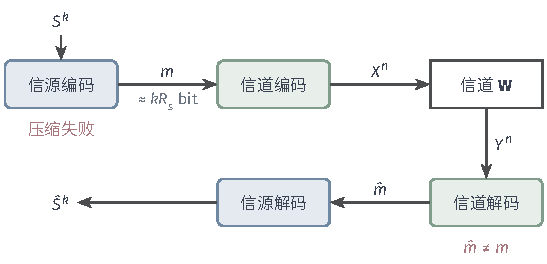
\includegraphics[width=92.7mm]{figures/07-probability/06-channel-coding/tikz/ccode-separation-pipeline/figure.pdf}
 \caption{分离的信源信道传输。$k$个源符号$S^{k}$经信源编码（蓝）变成编号$m$，约用$kR_{\mathrm{s}}$比特描述；信道编码（绿）把编号映成$n$个信道输入，经信道$\bm{W}$得到输出，信道解码给出编号的判决$\hat{m}$，信源解码给出重构$\hat{S}^{k}$。红字标出两种失败：信源编码本身失败，以及编号被判错。}
 \label{fig:ccode-separation-pipeline}
\end{BookInlineFigure}

下面先在无损要求下、再在失真要求下说明这一构造何时可行，以及任何方案（不论是否分离）都必须满足什么条件。若信道输入有逐码字的成本预算，第~\ref{chap:discrete-channel-capacity}章给出的受限容量与满足预算的码可以照样代入，下文的$C$换成对应的受限容量。

\subsection{无损传输}
\label{sec:ccode-lossless-transmission}

无损的要求是整块源符号被正确恢复的概率趋于$1$，此时$\hat{\mathcal{S}}=\mathcal{S}$。以下熵$H(S)$都以bit计。

\begin{theorem}[无损传输的分离定理]
\label{thm:ccode-lossless-separation}
设信源与信道如上，比例$r$满足式~\eqref{eq:ccode-ratio}。
\begin{enumerate}
 \item 若$rH(S)<C$，则存在一列分离方案，使
 \begin{equation}
  \mathbb{P}\bigl(\hat{S}^{k_n}\neq S^{k_n}\bigr)\to0 .
  \label{eq:ccode-lossless-goal}
 \end{equation}
 \item 若某一列联合信源信道编码（不必分离）满足式~\eqref{eq:ccode-lossless-goal}，则
 \begin{equation}
  rH(S)\leq C .
  \label{eq:ccode-lossless-converse}
 \end{equation}
\end{enumerate}
\end{theorem}

\paragraph{可达性的证明}
思路是在压缩与传输之间各留一点速率余量。因为$rH(S)<C$，可以选两个数$R_{\mathrm{s}}$与$R_{\mathrm{c}}$，使
\[
 H(S)<R_{\mathrm{s}},\qquad rR_{\mathrm{s}}<R_{\mathrm{c}}<C .
\]
先取$R_{\mathrm{s}}$略大于$H(S)$且$rR_{\mathrm{s}}<C$，再在$rR_{\mathrm{s}}$与$C$之间取$R_{\mathrm{c}}$。$R_{\mathrm{s}}$是信源编码的码率（每源符号的比特数），$R_{\mathrm{c}}$是信道编码的码率（每次使用的比特数）。

信源一侧，第~\ref{chap:lossless-coding}章的定长块编码可达性给出：对$R_{\mathrm{s}}>H(S)$，存在把$S^{k}$映成至多$2^{kR_{\mathrm{s}}}$个编号的定长编码，使不能正确还原的概率$\delta_k\to0$。信道一侧，第~\ref{chap:discrete-channel-capacity}章的编码定理给出：对$R_{\mathrm{c}}<C$，存在至少$2^{nR_{\mathrm{c}}}$条消息、最大错误概率$\lambda_{\max}^{(n)}\to0$的码。

两侧要能接上，编号的个数不能超过信道码的消息数。由$k_n/n\to r$与$rR_{\mathrm{s}}<R_{\mathrm{c}}$，$n$充分大时
\[
 k_nR_{\mathrm{s}}\leq nR_{\mathrm{c}} ,
\]
于是$2^{k_nR_{\mathrm{s}}}\leq2^{nR_{\mathrm{c}}}$。只使用信道码的前一部分消息即可；去掉的消息原来的判决区域可以并入任意保留的消息，保留消息的判决区域只增不减，所以最大错误概率不会变大。

整块恢复失败，只可能是信源编码失败或编号被判错，用并集上界：
\[
 \mathbb{P}\bigl(\hat{S}^{k}\neq S^{k}\bigr)\leq\delta_{k}+\mathbb{P}(\hat{m}\neq m) .
\]
信道噪声与信源独立，给定编号为$m$时判错的条件概率就是信道码的$\lambda_m$。编号的分布由信源决定，一般很不均匀，但无论它怎样分布，
\[
 \mathbb{P}(\hat{m}\neq m)=\sum_{m}\mathbb{P}(\text{编号}=m)\,\lambda_m\leq\lambda_{\max}^{(n)} .
\]
两项都趋于零，式~\eqref{eq:ccode-lossless-goal}成立。

这一步解释了为什么需要第~\ref{chap:discrete-channel-capacity}章的最大错误概率。若只知道均匀消息下的平均错误小，个别消息可能错误很大；而压缩后的编号恰好可能集中在这些消息上。逐消息的保证使信道码对任何编号分布都可靠。第~\ref{chap:discrete-channel-capacity}章删除坏码字的例子中，一个$16$条码字的随机码平均错误为$0.069$，最差的一条消息却达到$0.253$；若压缩后的编号恰好常常落在这条消息上，实际错误就接近$0.253$而不是$0.069$。

\paragraph{逆定理的证明}
现在设任一列联合编码满足式~\eqref{eq:ccode-lossless-goal}，把整块恢复失败的概率记作$P_{\mathrm{e}}^{(n)}$。信源无记忆，块的熵是单个熵的$k$倍，按熵与互信息的关系，
\[
 kH(S)=H(S^{k})=H(S^{k}\mid\hat{S}^{k})+I(S^{k};\hat{S}^{k}) .
\]

第一项用第~\ref{chap:information-measures}章的Fano不等式。$S^{k}$至多取$\lvert\mathcal{S}\rvert^{k}$个值，以bit计，
\[
 H(S^{k}\mid\hat{S}^{k})\leq1+P_{\mathrm{e}}^{(n)}\,k\log_2\lvert\mathcal{S}\rvert .
\]

第二项用数据处理不等式。编码器只看$S^{k}$，没有反馈，给定$X^{n}$后$Y^{n}$的条件分布不再依赖$S^{k}$，解码器只看$Y^{n}$，所以$S^{k}$、$X^{n}$、$Y^{n}$、$\hat{S}^{k}$按顺序构成Markov链。再用第~\ref{chap:discrete-channel-capacity}章的块互信息上界，
\[
 I(S^{k};\hat{S}^{k})\leq I(X^{n};Y^{n})\leq nC .
\]

两项相加，得到
\[
 kH(S)\leq1+P_{\mathrm{e}}^{(n)}\,k\log_2\lvert\mathcal{S}\rvert+nC .
\]
两边除以$n$，
\[
 \frac{k_n}{n}H(S)\leq\frac1n+P_{\mathrm{e}}^{(n)}\,\frac{k_n}{n}\log_2\lvert\mathcal{S}\rvert+C .
\]
令$n\to\infty$，$k_n/n\to r$，$P_{\mathrm{e}}^{(n)}\to0$，就得到式~\eqref{eq:ccode-lossless-converse}。

逆定理没有假设编码是分离的，它对任何把信源和信道合在一起的设计都成立。所以在$rH(S)\neq C$的地方，分离方案与最好的联合方案有相同的可行范围：分离在渐近意义下不损失任何速率。

\paragraph{例子}
回到开头的雨天记录，$P_S=\operatorname{Bern}(0.1)$，信道是$p=0.1$的二元对称信道：
\[
 H(S)=h_2(0.1)\approx0.469,\qquad C=1-h_2(0.1)\approx0.531 .
\]
定理给出的界限是
\[
 r<\frac{C}{H(S)}\approx1.13 .
\]
也就是说，每次信道使用可以可靠地传送约$1.13$个源比特，多于一个。不压缩而直接把源比特当作消息比特送进信道码，只能做到$r<C=0.531$。特别地，$r=1$时$rH(S)=0.469<0.531$，可以让每次信道使用传送一个源比特而几乎不出错；直接发送则有$10\%$的比特出错。图~\ref{fig:ccode-lossless-budget}画出不同信源参数下的界限：信源越可预测，压缩带来的收益越大。

\begin{BookInlineFigure}
 \centering
 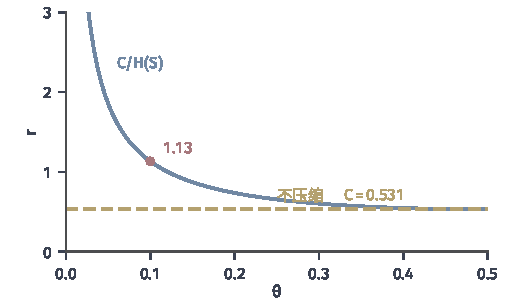
\includegraphics[width=86mm]{figures/07-probability/06-channel-coding/matplotlib/ccode-lossless-budget/figure.pdf}
 \caption{$\operatorname{Bern}(\theta)$信源经$p=0.1$的二元对称信道无损传输时，每次信道使用可传送的源符号数$r$的上限。蓝线为$C/H(S)=C/h_2(\theta)$，红点为$\theta=0.1$时的$1.13$；黄色虚线为不压缩时的上限$C=0.531$。$\theta=\tfrac12$时信源已无冗余，两者相等。}
 \label{fig:ccode-lossless-budget}
\end{BookInlineFigure}

\subsection{有损传输}
\label{sec:ccode-lossy-transmission}

许多信源不必精确恢复，只要重构的平均失真不超过某个水平。这时信源一侧用第~\ref{chap:rate-distortion}章的率失真编码代替无损压缩。

\paragraph{设定}
设重构字母表$\hat{\mathcal{S}}$有限，失真函数有界：
\[
 d:\mathcal{S}\times\hat{\mathcal{S}}\to[0,d_{\max}] .
\]
块的失真取逐符号平均
\[
 d_k(s^{k},\hat{s}^{k})=\frac1k\sum_{i=1}^{k}d(s_i,\hat{s}_i) .
\]
要求是渐近期望失真不超过$D$：
\begin{equation}
 \limsup_{n\to\infty}\mathbb{E}\bigl[d_{k_n}(S^{k_n},\hat{S}^{k_n})\bigr]\leq D .
 \label{eq:ccode-lossy-goal}
\end{equation}
这里的$R(D)$是第~\ref{chap:rate-distortion}章的信息率失真函数：在满足$\mathbb{E}\,d(S,\hat{S})\leq D$的测试信道中，互信息$I(S;\hat{S})$的下确界。那里证明了它非增、凸，在取有限值的区间上连续，并且等于渐近期望失真下的最低描述率。

\begin{theorem}[有损传输的分离定理]
\label{thm:ccode-lossy-separation}
在上述设定下：
\begin{enumerate}
 \item 若$rR(D)<C$，则存在一列分离方案满足式~\eqref{eq:ccode-lossy-goal}。
 \item 若某一列联合信源信道编码满足式~\eqref{eq:ccode-lossy-goal}，则
 \begin{equation}
  rR(D)\leq C .
  \label{eq:ccode-lossy-converse}
 \end{equation}
\end{enumerate}
\end{theorem}

\paragraph{可达性的证明}
与无损情形一样留出余量：取$R_{\mathrm{s}}'>R_{\mathrm{s}}>R(D)$与$R_{\mathrm{c}}$，使
\[
 rR_{\mathrm{s}}'<R_{\mathrm{c}}<C .
\]
由第~\ref{chap:rate-distortion}章的率失真编码定理，$(R_{\mathrm{s}},D)$是可达码率失真对：存在一列率失真码，码率的上极限不超过$R_{\mathrm{s}}$，期望失真的上极限不超过$D$。于是$k$充分大时，编号个数$M_k\leq2^{kR_{\mathrm{s}}'}$。信道一侧与无损情形相同，取最大错误概率$\lambda_{\max}^{(n)}\to0$的信道码，$n$充分大时编号能够放进去。

失真按两种情形分开估计。编号被正确判出时，重构就是率失真码本身的重构，失真与不经过信道时相同；编号被判错时，重构是另一条码字，失真不超过$d_{\max}$。所以
\[
 \mathbb{E}\bigl[d_k(S^{k},\hat{S}^{k})\bigr]\leq\mathbb{E}\bigl[d_k\bigl(S^{k},g_k(f_k(S^{k}))\bigr)\bigr]+d_{\max}\,\lambda_{\max}^{(n)} ,
\]
其中$f_k,g_k$是率失真码的编码与重构。第一项的上极限不超过$D$，第二项趋于零，式~\eqref{eq:ccode-lossy-goal}成立。有界失真在这里起关键作用：信道偶尔出错时，造成的额外失真被$d_{\max}$乘以一个趋于零的概率控制住。

\paragraph{逆定理的证明}
设$D_k=\mathbb{E}[d_k(S^{k},\hat{S}^{k})]$，$D_{k,i}=\mathbb{E}[d(S_i,\hat{S}_i)]$，于是$D_k$是$D_{k,i}$对$i$的平均。先给互信息一个下界。由链式法则与源符号的独立性，
\[
 I(S^{k};\hat{S}^{k})=H(S^{k})-H(S^{k}\mid\hat{S}^{k})=\sum_{i=1}^{k}H(S_i)-H(S^{k}\mid\hat{S}^{k}) .
\]
条件熵满足次可加性，并且多加条件不会增加熵，所以
\[
 H(S^{k}\mid\hat{S}^{k})\leq\sum_{i=1}^{k}H(S_i\mid\hat{S}^{k})\leq\sum_{i=1}^{k}H(S_i\mid\hat{S}_i) .
\]
代回，得到
\[
 I(S^{k};\hat{S}^{k})\geq\sum_{i=1}^{k}I(S_i;\hat{S}_i) .
\]

每一对$(S_i,\hat{S}_i)$的联合分布中，$S_i\sim P_S$，给定$S_i$时$\hat{S}_i$的条件分布是一个平均失真为$D_{k,i}$的测试信道，所以$I(S_i;\hat{S}_i)\geq R(D_{k,i})$。再由$R$的凸性（Jensen不等式），
\[
 \sum_{i=1}^{k}R(D_{k,i})\geq kR\Bigl(\frac1k\sum_{i=1}^{k}D_{k,i}\Bigr)=kR(D_k) .
\]
另一方面，与无损情形相同的Markov链与块互信息上界给出$I(S^{k};\hat{S}^{k})\leq nC$。合起来，
\[
 \frac{k_n}{n}\,R(D_{k_n})\leq C .
\]

最后取极限。任取$\eta>0$，由式~\eqref{eq:ccode-lossy-goal}，$n$充分大时$D_{k_n}\leq D+\eta$；$R$非增，所以
\[
 R(D+\eta)\leq R(D_{k_n})\leq\frac{n}{k_n}C\to\frac Cr .
\]
于是对每个$\eta>0$都有$rR(D+\eta)\leq C$。若$D$低于最小可行失真$D_{\min}$，任何重构都有$D_k\geq D_{\min}$，式~\eqref{eq:ccode-lossy-goal}不可能成立，所以只需考虑$D\geq D_{\min}$，此时$R(D)$有限。第~\ref{chap:rate-distortion}章证明了$R$在$[D_{\min},\infty)$上连续（包括左端点），令$\eta\downarrow0$，就得到式~\eqref{eq:ccode-lossy-converse}。

\paragraph{例子：均匀二元信源}
设$P_S=\operatorname{Bern}(\tfrac12)$，Hamming失真，信道仍是$p=0.1$的二元对称信道。由第~\ref{chap:rate-distortion}章，
\[
 R(D)=1-h_2(D),\qquad 0\leq D\leq\tfrac12 .
\]
给定$r$，能达到的最小失真$D^{*}(r)$由$rR(D)=C$决定：$r\leq C$时任何正失真都可以达到（无损传输的条件$rH(S)=r<C$在$r<C$时就已满足）；$r>C$时
\begin{equation}
 D^{*}(r)=h_2^{-1}\Bigl(1-\frac Cr\Bigr) ,
 \label{eq:ccode-dstar}
\end{equation}
其中$h_2^{-1}$是$h_2$在$[0,\tfrac12]$上的反函数。$r=1$时$1-C=h_2(0.1)$，所以
\[
 D^{*}(1)=0.1 .
\]
$r=2$时$1-C/2\approx0.735$，$D^{*}(2)\approx0.206$。

图~\ref{fig:ccode-lossy-tradeoff}把这条曲线与几个具体方案放在一起。三次与五次重复码的$r$分别为$\tfrac13$与$\tfrac15$，每个源比特的错误率是$0.028$与$0.0086$，而在这些$r$上理论上可以把失真压到任意小。Hamming码在$r=\tfrac47$处的比特错误率是$0.067$，界限是$0.0085$。$r=2$时，“发送一个比特、另一个猜”的失真是$(0.1+0.5)/2=0.3$，界限是$0.206$。最引人注意的是$r=1$：把源比特原样送进信道，不做任何编码，失真正好是$0.1$，恰好落在界限上。

\begin{BookInlineFigure}
 \centering
 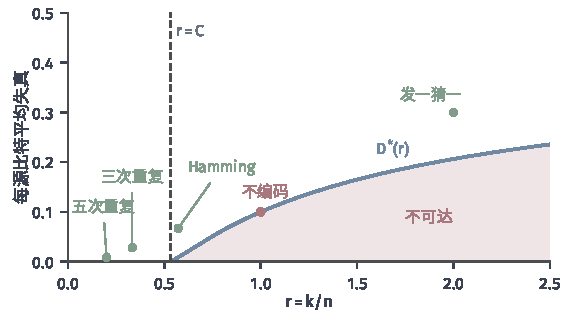
\includegraphics[width=96mm]{figures/07-probability/06-channel-coding/matplotlib/ccode-lossy-tradeoff/figure.pdf}
 \caption{均匀二元信源、Hamming失真、$p=0.1$的二元对称信道。蓝线为式~\eqref{eq:ccode-dstar}的最小可达失真$D^{*}(r)$（$r\leq C$时为$0$），其下方的红色区域被逆定理排除；虚线为$r=C$。绿点为具体方案的精确值：五次重复、三次重复、$[7,4,3]$ Hamming码的比特错误率，以及$r=2$时发一个比特、猜另一个。红点为不编码直接发送，$r=1$，失真$0.1$。}
 \label{fig:ccode-lossy-tradeoff}
\end{BookInlineFigure}

\subsection{分离原则的范围}
\label{sec:ccode-separation-scope}

两条分离定理说：在规定的条件下，比较$rH(S)$或$rR(D)$与$C$这两个数，就决定了传输能否成功，并且分开设计足以达到这个界限。这个结论的每一部分都附带条件，去掉条件，结论就可能失效或需要另行论证。

\paragraph{严格不等式与渐近}
可达性需要严格不等式$rR(D)<C$，因为证明要在压缩与传输两侧各留一点余量；逆定理只给出非严格的$rR(D)\leq C$。在等号$rR(D)=C$处，定理既不保证可以做到，也不保证做不到。而且两边都是块长趋于无穷的陈述：它们不承诺某个有限的块长已经足够，不承诺零错误，也不承诺失真恰好等于$D$。第~\ref{sec:ccode-finite}节已经看到，单是信道一侧，块长$1000$就要比容量多付出约$16\%$的码率；分离方案在信源一侧还有另一份有限块的损失。

\paragraph{联合方案可以更简单}
上面均匀二元信源的例子中，不编码直接发送在$k=n=1$、没有任何延迟的情况下就达到了$D^{*}(1)=0.1$；分离方案要接近同一失真，两侧的块长都必须很长。原因是这个信源与信道恰好“匹配”：均匀的源比特正是使二元对称信道达到容量的输入分布，信道的翻转又恰好产生信源所需的Hamming失真。分离定理说分开设计不吃亏，不是说分开设计是唯一的好办法；在有限延迟下，匹配的联合方案可以严格优于有限块长的分离方案。

\paragraph{高斯信源与无界失真}
同样的匹配也出现在连续的情形。设信源$S\sim\mathcal{N}(0,\sigma_S^{2})$，信道是$Y=X+Z$，$Z\sim\mathcal{N}(0,\sigma_Z^{2})$与输入独立，输入功率不超过$P_{\mathrm{s}}$（这里用$P_{\mathrm{s}}$表示功率，以免与概率混淆）。每次使用传送一个源符号，即$r=1$。

不编码时发送$X=aS$，其中$a=\sqrt{P_{\mathrm{s}}/\sigma_S^{2}}$使功率恰为$P_{\mathrm{s}}$，接收端用$\mathbb{E}[S\mid Y]$估计$S$。$(S,Y)$是联合高斯的，$\operatorname{Cov}(S,Y)=a\sigma_S^{2}$，$\operatorname{Var}(Y)=P_{\mathrm{s}}+\sigma_Z^{2}$，最优估计$\mathbb{E}[S\mid Y]$是$Y$的线性函数，它的均方误差是条件方差：
\[
 \begin{aligned}
 \operatorname{Var}(S\mid Y)&=\sigma_S^{2}-\frac{\operatorname{Cov}(S,Y)^{2}}{\operatorname{Var}(Y)}=\sigma_S^{2}-\frac{a^{2}\sigma_S^{4}}{P_{\mathrm{s}}+\sigma_Z^{2}}\\
 &=\sigma_S^{2}-\frac{P_{\mathrm{s}}\sigma_S^{2}}{P_{\mathrm{s}}+\sigma_Z^{2}}=\frac{\sigma_S^{2}\sigma_Z^{2}}{P_{\mathrm{s}}+\sigma_Z^{2}} .
 \end{aligned}
\]

另一方面，第~\ref{chap:rate-distortion}章的高斯率失真函数与第~\ref{chap:gaussian-channel-capacity}章的高斯信道容量给出$r=1$时的界限
\[
 \frac12\log_2\frac{\sigma_S^{2}}{D}\leq\frac12\log_2\Bigl(1+\frac{P_{\mathrm{s}}}{\sigma_Z^{2}}\Bigr) ,
\]
即
\[
 D\geq\frac{\sigma_S^{2}\sigma_Z^{2}}{P_{\mathrm{s}}+\sigma_Z^{2}} .
\]
不编码再次恰好达到界限。

但这里的分离定理不能照搬上面的证明。平方失真$(s-\hat{s})^{2}$无界，可达性证明中“信道出错时失真不超过$d_{\max}$”这一步失效：编号被判错时，重构可能离信源很远，额外的失真不再被一个趋于零的概率乘以常数所控制。要沿用分离构造，必须另外控制信道出错事件上的失真，例如限制重构值的范围并利用信源的二阶矩证明这部分期望趋于零。字母表也不再有限，率失真编码与信道编码本身都要用连续情形的定理。

\paragraph{记忆与有限延迟}
本节的信源与信道都是无记忆的，块长可以任意增长。若信源相邻符号相关，或信道的噪声随时间相关，熵和容量都要换成按单位时间计算的极限量，这些极限是否存在、是否等于可操作的速率，取决于过程的平稳性与遍历性一类条件，需要随机过程的工具另行建立。若应用要求有限延迟，块长不能任意增长，就需要直接核算有限块的代价。在这些情形下，只比较两个标量速率并沿用全部结论是不够的。
